\documentclass[10pt,twocolumn,letterpaper]{article}

\usepackage{cvpr}
\usepackage{times}
\usepackage{epsfig}
\usepackage{graphicx}
\usepackage{amsmath}
\usepackage{amssymb}

% Include other packages here, before hyperref.

% If you comment hyperref and then uncomment it, you should delete
% egpaper.aux before re-running latex.  (Or just hit 'q' on the first latex
% run, let it finish, and you should be clear).
\usepackage[breaklinks=true,bookmarks=false]{hyperref}

\cvprfinalcopy % *** Uncomment this line for the final submission

\def\cvprPaperID{****} % *** Enter the CVPR Paper ID here
\def\httilde{\mbox{\tt\raisebox{-.5ex}{\symbol{126}}}}

% Pages are numbered in submission mode, and unnumbered in camera-ready
%\ifcvprfinal\pagestyle{empty}\fi
\setcounter{page}{1}
\begin{document}

%%%%%%%%% TITLE
\title{Milestone: Supervised Learning of Multiplicative Semantic Word Embeddings from Semantic Entailment Data}

\author{Ao Liu\\
University of Massachusetts Amherst\\
140 Governors Dr., Amherst, MA 01003 \\
{\tt\small aoliu@umass.edu}
% For a paper whose authors are all at the same institution,
% omit the following lines up until the closing ``}''.
% Additional authors and addresses can be added with ``\and'',
% just like the second author.
% To save space, use either the email address or home page, not both
}

\maketitle
%\thispagestyle{empty}

%%%%%%%%% ABSTRACT
%\begin{abstract}
%
%\end{abstract}

%%%%%%%%% BODY TEXT
\section{Introduction}
Many natural language processing (NLP) tasks rely word embeddings. Traditionally, word embeddings are trained unsupervisedly on large corpus. This approach has in general worked well on many NLP related tasks. However, implementations of this unsupervised approach usually focus on the syntactic representations of words, thus lack of semantic interpretations. Syntactic representations usually follow additive rules, i.e. "king" - "man" + "woman" = "queen". One of the problem is syntactic representations can hardly deal with negation and degree modifiers. Research shows that multiplicative embeddings perform better on semantic tasks, such as entailment. As an important task of semantics, entailment teaches the computer how to understand the meaning of a sentence and the implicit idea behind it. I want to find a supervised way to train multiplicative semantic word embeddings with the help of paraphrase/entailment dataset(s). Due to the change on embeddings, I will also implement a new entailment model architecture better fitting the multiplicative property of the presented word embeddings.

\section{Problem Statement}
Distributed representations of words (or word Embeddings)\cite{bengio2003neural, collobert2011natural, mikolov2013distributed, pennington2014glove} are generally used for many NLP tasks in recent years. Although these unsupervisedly trained word embeddings are capable of finding the general topic in a sentence based on the syntactic relationships of words, they still lack of semantic interpretations. Due to this problem, it is hard to find meaningful representation of a full sentence. A most recent paper shows that capturing the relationships among multiple words and phrases in a single vector to form the sentence representation can improve the performance on semantic entailment tasks \cite{conneau2017supervised}. However, the provided method using syntax-based word embeddings may still have ignored the impact of semantic meanings of words.

There are two major families of unsupervisedly learning wrod embeddings: 1) global matrix factorization methods, such as latent semantic analysis (LSA) \cite{deerwester1990indexing} 2) co-occurrence methods, such as skip-gram model of Mikolov \etal \cite{mikolov2013distributed} and global log-bilinear regression model of Pennington \etal \cite{pennington2014glove}. Pennington \etal seem better statistically solving global information, but the problem of semantics interpretation remain unsolved. Some significant examples are around 1) negation words, such as "not" and 2) degree modifiers, such as "more" and "less". Those examples are problematic because such negation words or degree modifiers can be added to any syntactically completed sentences, but the semantic meaning of the sentence may be altered for a certain degree. Training such words in an unsupervised manner is unwise and usually result in meaningless representations.

In my project, I try to study the task of learning semantic word embeddings that is trained on a large corpus in order to relieve some difficulties of finding more general semantic sentence representations. To obtain such semantic word embeddings, two major problem need to be solved, namely: what would be a suitable neural network architecture; and how and on what task should such a network be trained. Most approaches of existing work on learning word embeddings in an unsupervised maner like word2vec \cite{mikolov2013distributed} and GloVe \cite{pennington2014glove}. I want to see if supervised learning can help solving the problem. The idea is inspired by previous result in NLP, where Alexis Conneau \etal train universal sentence representation \cite{conneau2017supervised}, and in computer vision, where researchers pretrain models on the ImageNet \cite{deng2009imagenet} and transfer the learned features to other tasks. Conneau \etal show that training sentence embeddings on a natural language inference (NLI) task achieve the best transferability \cite{conneau2017supervised}. The reason is that NLI is a high-level understanding task involving reasoning about the semantic relationships within sentences. Hence, I hypothesize that such task can also help training semantic word embeddings.

There are mainly two datasets that I may use. One is the Stanford Natural Language Inference (SNLI) corpus \cite{bowman2015large}, which is a collection of 570k human-written English sentence pairs manually labeled for balanced classification with the labels entailment, contradiction, and neutral, supporting the task of natural language inference (NLI), also known as recognizing textual entailment (RTE). The other is Paraphrase Database (PPDB) \cite{ganitkevitch2013ppdb}, which is an extensive semantic resource, consisting of a list of phrase pairs with (heuristic) confidence estimates. The dataset to be used may vary, depending on further exploration and understanding on them.

Unlike in computer vision, where convolutional neural networks (CNNs) dominate the field, many architectures are used in NLP tasks. I want to investigate the impact of various semantic entailment architectures using neural networks and compare their performances on top of the learned semantic word embeddings. The models will be evaluated on the accuracy of the entailment task, \ie the percentage of correctly inferred relationship of sentence pairs in the dataset.

\section{Technical Approach}
This work combines two research directions. First, I explain how the NLI task can be used to train semantic word embeddings using the SNLI task. Then I describe the architectures that I investigate for the entailment model. Specifically, I examine standard recurrent models such as LSTMs \cite{hochreiter1997long} and CNNs.

\subsection{The Natural Language Inference Task}
There are 570k human-written English sentence pairs labelled with one of the three categories: entailment, contradiction, and neutral. It captures NLI, or RTE, and is one of the largest high-quality labelled dataset for semantics related NLP training purpose. I hypothesize that the semantic nature of NLI makes it a good candidate for learning semantic word embeddings in a supervised way. That is, I want to show that semantic word embeddings trained on NLI are able to capture the semantic meaning of words and can potentially improve the performance of entailment systems.

There are two ways to train the word embeddings on SNLI: 1) adapt word co-occurrence statistics and 2) train embeddings of words in a sentence pair simultaneously.

\begin{figure}[ht]
\begin{center}
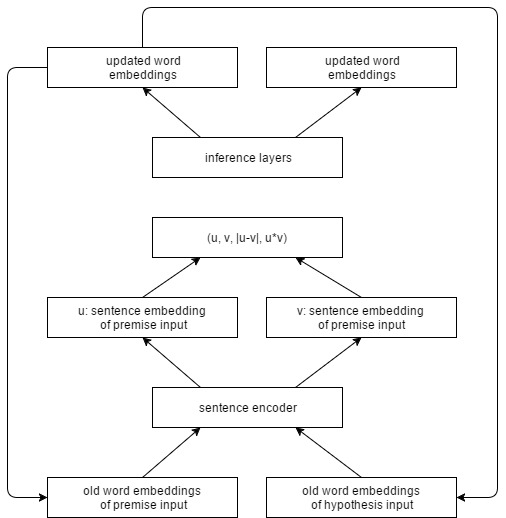
\includegraphics[scale=0.5]{model_architecture}
\end{center}
\caption{A generic architecture of learning word embeddings on SNLI in a supervised manner}
\label{fig:model_arc}
\end{figure}

Since training word embeddings within sentence pairs simultaneously implicitly shows the co-occurrences of words, I adopt the second setting. As illustrated in Figure \ref{fig:model_arc}, a typical architecture of this kind trains word embeddings of sentence pairs simultaneously. The word embeddings of premise and hypothesis inputs are passed through a shared sentence encoder to obtain the sentence embeddings premise $u$ and hypothesis $v$. Once the sentence embeddings are generated, 3 matching methods are applied to extract relations between $u$ and $v$: 1) concatenation of $u$ and $v$, 2) element-wise absolute difference $|u - v|$ and 3) element-wise product $u*v$. The resulting vector will contain informations from both $u$ and $v$ and then be passed into inference layer(s) along with a softmax output layer. This will simultaneously update all the embeddings of words in the sentence pair and the updated word embeddings will then be applied to the following training iterations.

\subsection{Sentence Entailment Architectures}
Various neural networks for NLI exist. However, current systems are usually based on pre-trained word embeddings using unsupervised techniques. The architecture that better fits the semantic word embeddings is not yet clear. I want to compare different architectures: standard recurrent encoders with LSTMs or Bi-LSTMs, fully connected layers and even CNNs. 

\section{Intermediate Result}
Conneau \etal public their PyTorch implementation of their sentence encoder on GitHub \cite{conneau2017supervised}. For convenience of my implementation, I reimplement their work in TensorFlow and achieve similar results on SNLI (See Table \ref{tab:entail_acc}).

\begin{table}[ht]
\begin{center}
\begin{tabular}{|l|c|c|c|}\hline
Model		& dim	& dev	& test \\\hline
LSTM		& 2048	& 81.9	& 80.7 \\\hline
GRU			& 4096	& 82.4	& 81.8 \\\hline
BiGRU-last	& 4096	& 81.3	& 80.9 \\\hline
BiLSTM-mean	& 4096	& 79.0	& 78.2 \\\hline
BiLSTM-Max	& 4096	& 85.0	& 84.5 \\\hline
\end{tabular}
\end{center}
\caption{Performance of sentence encoder architectures on SNLI. Dimensions of embeddings were selected according to best aggregated scores.}
\label{tab:entail_acc}
\end{table}

{\small
\bibliographystyle{unsrt}
\bibliography{milestone}
}

\end{document}
